\documentclass[a4paper,10pt]{article}
\usepackage[utf8x]{inputenc}

\usepackage{amsmath}    % need for subequations
\usepackage{graphicx}   % need for figures
\usepackage{verbatim}   % useful for program listings
\usepackage{color}      % use if color is used in text
\usepackage{subfigure}  % use for side-by-side figures
\usepackage{hyperref}   % use for hypertext links, including those to external documents and URLs
\usepackage{cancel} 
\usepackage{titlesec}
\usepackage{array} 	% use for creating arrays such as eqnarray
\usepackage{float}	% Float for Sourcecode
\usepackage{listings}

\setlength{\parskip}{3pt plus 2pt}
\setlength{\parindent}{20pt}

\setlength{\oddsidemargin}{-0.6in}
%\setlength{\evensidemargin}{0.5cm}
%\setlength{\marginparsep}{0.75cm}
%\setlength{\marginparwidth}{2.5cm}
%\setlength{\marginparpush}{1.0cm}
\setlength{\textwidth}{7.4in}
%\headheight{1in}
%\topmargin{0.5in}
%\textheight{10.0in}
%\footheight{0.1in} 


% Colors
\definecolor{headertextcolor}{rgb}{.88,.65,.11}
\definecolor{headerboxcolor}{rgb}{.88,.65,.11}



% Header style
\titleformat{\section}{\color{headertextcolor}\large\scshape\raggedright}{}{0em}{}[\titlerule]
\titleformat{\subsection}{\color{headertextcolor}\normalfont\normalsize\bfseries}{}{0em}{}[]
\titleformat{\mbox}{\color{headertextcolor}}{}{}{}

\floatstyle{ruled}
\newfloat{program}{thp}{lop}
\floatname{program}{Program}


%opening
\title{FDTD Sources}
\author{Christopher Stricklan}
\date{Revised: February 21, 2011}



\begin{document}

\maketitle

\begin{abstract}
This document describes and formulates the various sources that can be used in FDTD models. 
\end{abstract}

\vfill


\section{1D Sources}
\subsection{Gaussian Pulse}
The Gaussian Pulse is an impulse function that allows us to excite the problem with a broad range of frequencies all at the same time.

\begin{figure}[ht]
  \label{fig:GaussianPulse}
   \centering
     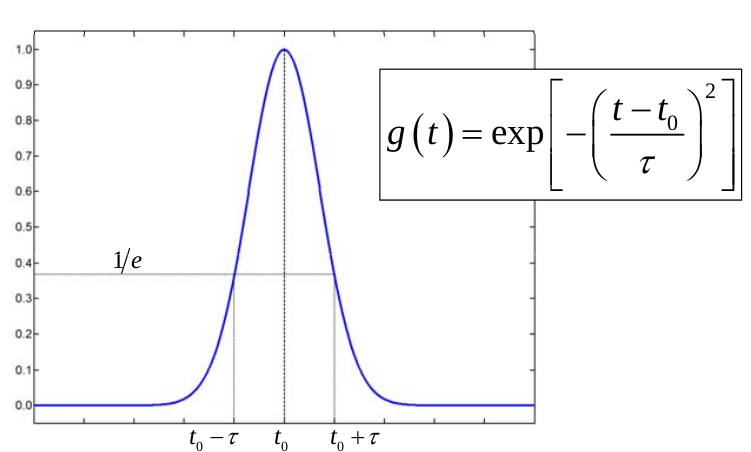
\includegraphics[width=0.75\textwidth]{GaussianPulse.png}
   \caption{A Gaussian Pulse centered at $t_0$}
\end{figure}

To find the frequency content of the Pulse we must perform the Fourier Transform on the pulse.  

\begin{equation*}
  g(t) = \exp\left(-\frac{t^2}{\tau^2}\right) \Longrightarrow G(f) = \frac{1}{\sqrt{\pi}B}\exp\left[-\frac{f^2}{B^2}\right] 
\end{equation*}

This shows that the frequency content of the Gaussian Pulse extends from DC up to B where

\begin{equation}
 B = \frac{1}{\pi\tau}
\end{equation}

\textbf{Pulse Design}

To design the pulse for our simulations we must first decide on the maximum frequency we are interested in $f_{max}$ then compute the pulse width with this upper frequency

\begin{equation*}
 B = f_{max}=\frac{1}{\pi\tau} \Longrightarrow \tau \leq \frac{1}{\pi f_{max}}
\end{equation*}

For simplification we can approximate $\tau$ as

\begin{equation}
 \tau \cong \frac{0.5}{f_{max}}
\end{equation}

In order to properly resolve our Guassian pulse, which should be completed by at least 10 to 20 time steps, we need to recalculate $\Delta t$.  We now need  to re-evaluate this value in conjuction with the Courant Stability Condition.  We will determine $\Delta t$ based on the maximum frequency and pick the smallest $\Delta t$.

\begin{equation}
 \Delta t \leq \frac{\tau}{10}
\end{equation}

Finally to properly inject our source without any adverse reactions within our model we must include delay \ref{fig:GaussianPulseDelay}.  This will allow the pulse to ease into the problem space without producing large field gradients.

\begin{equation}
 t_0 \geq 6\tau
\end{equation}

\begin{figure}[ht]
  \label{fig:GaussianPulseDelay}
   \centering
     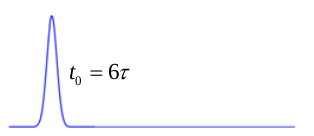
\includegraphics[width=0.5\textwidth]{GaussianPulseDelay.png}
   \caption{A Gaussian Pulse delayed by $t_0 = 6\tau$}
\end{figure}


\textbf{Matlab Example}





\begin{program}
  \lstset{language=Matlab}
  \lstinputlisting{code/GaussianSource.m}
  \caption{The Gaussian Source Example}
\end{program}









\end{document}


